% Note on compiling: requires external programs dot (from the graphvix package
% on Debian/Ubuntu) and dot2tex.
% You need to pass the --shell-escape option to pdflatex
% (or use the Makefile, which required latexmk).
%\documentclass[aspectratio=169,handout]{beamer}
%\documentclass[aspectratio=169,handout,hyphens]{beamer} % hyphens option for url package which beamer loads.
\documentclass[aspectratio=169,hyphens]{beamer} % hyphens option for url package which beamer loads.

\def\UrlFont{\small\tt}

\usepackage{minted}
\usepackage{color}
%\usepackage[pgf,dot]{dot2texi}
%\usepackage{tikz}
%\usetikzlibrary{shapes,arrows}

\usetheme{Pittsburgh}
\usecolortheme{beaver}
% \useoutertheme{infolines}

\title{Constraint Programming in Haskell}
\subtitle{Melbourne Haskell Users Group}
\author{David Overton}
\date{29 October 2015}

\AtBeginSection[]
{
	\begin{frame}
		\frametitle{Table of Contents}
		\tableofcontents[currentsection]
	\end{frame}
}

%\lstnewenvironment{code}{\lstset{language=Haskell,basicstyle=\small}}{}

\newminted[code]{haskell}{fontsize=\small}
\newmint[hask]{haskell}{fontsize=\small}
\newminted{prolog}{fontsize=\small}

\definecolor{mygreen}{rgb}{0,0.6,0}
\definecolor{mygrey}{rgb}{0.5,0.5,0.5}
\definecolor{mymauve}{rgb}{0.58,0,0.82}

\newtheorem{observation}[theorem]{Observation}

\newcommand\myheading[1]{%
  \par\bigskip
  {\large\color{blue}#1}\par\smallskip}
\begin{document}

\frame{\titlepage}

\section{Constraint programming}

\begin{frame}
    \frametitle{Constraint programming}
    Constraint programming is a declarative programming paradigm for solving constraint satisfaction problems.
    \pause
    \begin{itemize}
        \item A set of \emph{constraint variables} over a \emph{domain}, e.g. Booleans, integers, reals, finite domain.
        \item A set of \emph{constraints} between those variables.
        \item A \emph{solver} to find solutions to the constraints, i.e. assignments of variables to values in the domain such that all constraints are satisfied.
    \end{itemize}
    \pause
    Applications: planning, scheduling, resource allocation, computer graphics, digital circuit design, programming language analysis, \ldots
\end{frame}

\section{Constraint logic programming}

\begin{frame}
    \frametitle{Constraint logic programming}
    \begin{itemize}
        \item Constraint programming and logic programming work well together.
        \item Many Prolog implementations have built in constraint solvers.
        \item Basic idea:
            \begin{itemize}
                \item add constraints to the constraint store
                \item constraint solver works behind the scenes to propagate constraints
                \item use Prolog's backtracking search mechanism to generate solutions
            \end{itemize}
        \item Advantages over pure logic programming:
            \begin{itemize}
                \item ``constrain-and-generate'' rather than ``generate-and-test''
                \item constraint solver can greatly reduce the search space required compared to Prolog's built-in depth-first-search
                \item much more powerful than relying on just unification and backtracking
            \end{itemize}
    \end{itemize}
\end{frame}

\section{Finite domain constraints}

\begin{frame}[fragile]
    \frametitle{Finite domain constraints}
\begin{itemize}
    \item One of the most widely used varieties of constraint solver.
        \pause
    \item Variables range over a finite domain of integers.
        \pause
    \item Simple equality and inequality constraints: $=$, $\neq$, $<$, $>$, $\leq$, $\geq$
        \pause
    \item Also simple arithmetic expressions: $+$, $-$, $\times$, \texttt{abs}
\end{itemize}
\end{frame}

\begin{frame}[fragile]
    \frametitle{Arc consistency}
Solver uses an \emph{arc consistency algorithm}, e.g.\ AC-3
\begin{itemize}
    \item Constraint store holds the set of constraints to be checked.
        \pause
    \item For each constraint, the domains of the variables involved are checked to
        ensure they are consistent with the contraint.
        \pause
    \item Any values in the domains that break consistency are removed.
        \pause
    \item If the domain of a variable changes then all other constraints involving that variable are
        rechecked.
\end{itemize}
\pause
\begin{example}
\begin{displaymath}
    \begin{array}{c}
    x \in \{1, 2, 3\} ~~\land~~ y \in \{1, 2, 3\} \\
    \pause
    \textrm{add constraint~} x < y \\
    \pause
    \Rightarrow ~~~ x \in \{1, 2\} ~~\land~~ y \in \{2, 3\} \\
    \pause
    \textrm{add constraint~} y = 2 \\
    \pause
        \Rightarrow ~~~ x \in \{1\} ~~\land~~ y \in \{2\}
    \end{array}
\end{displaymath}
\end{example}
\end{frame}

\begin{frame}[fragile]
    \frametitle{Example: $n$ queens in SWI-Prolog}

\begin{columns}[t]
\column[c]{0.35\paperwidth}
\begin{minted}[fontsize=\small]{prolog}
n_queens(N, Qs) :-
        length(Qs, N),
        Qs ins 1..N,
        safe_queens(Qs).

safe_queens([]).
safe_queens([Q|Qs]) :-
    safe_queen(Qs, Q, 1),
    safe_queens(Qs).

safe_queen([], _, _).
safe_queen([Q|Qs], Q0, D0) :-
        Q0 #\= Q,
        abs(Q0 - Q) #\= D0,
        D1 #= D0 + 1,
        safe_queen(Qs, Q0, D1).
\end{minted}
\column[c]{0.5\paperwidth}
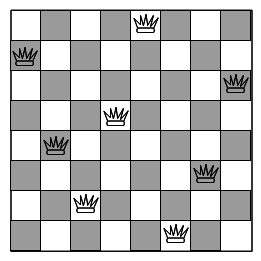
\includegraphics[width=0.45\paperwidth]{8queens.png}
\end{columns}
\end{frame}

\section{Constraint programming in Haskell}

\subsection{Basic equality and inequality}

\begin{frame}[fragile]
    \frametitle{Constraint programming in Haskell}
How can we do something similar in Haskell?\pause{}
\textbf{Use a monad!}
\end{frame}

\begin{frame}[fragile]
    \frametitle{Example: $n$ queens in SWI-Prolog and Haskell}

\begin{columns}[t]
\column[t]{0.33\paperwidth}
\begin{minted}[fontsize=\footnotesize]{prolog}
n_queens(N, Qs) :-
        length(Qs, N),
        Qs ins 1..N,
        safe_queens(Qs).

safe_queens([]).
safe_queens([Q|Qs]) :-
    safe_queen(Qs, Q, 1),
    safe_queens(Qs).

safe_queen([], _, _).
safe_queen([Q|Qs], Q0, D0) :-
        Q0 #\= Q,
        abs(Q0 - Q) #\= D0,
        D1 #= D0 + 1,
        safe_queen(Qs, Q0, D1).
\end{minted}
\pause
\column[t]{0.59\paperwidth}
\begin{minted}[fontsize=\footnotesize]{haskell}
nQueens :: Int -> FD [FDExpr]
nQueens n = do
    qs <- news n (1, n)
    safeQueens qs
    return qs

safeQueens :: [FDExpr] -> FDConstraint
safeQueens [] = return ()
safeQueens (q : qs) = do
    safeQueen qs q 1
    safeQueens qs

safeQueen :: [FDExpr] -> FDExpr -> FDExpr -> FDConstraint
safeQueen [] _ _ = return ()
safeQueen (q : qs) q0 d0 = do
   q0 #\= q 
   abs (q0 - q) #\= d0
   safeQueen qs q0 (d0 + 1)
\end{minted}
\end{columns}
\end{frame}
\begin{frame}[fragile]
\begin{itemize}
    \item List monad provides backtracking / search / multiple solutions.
        \pause
    \item Wrap it in a state monad transformer to keep track of the constraint store.
        \pause
\end{itemize}
\begin{code}
type FD a = StateT FDState [] a
\end{code}
\pause
\begin{code}
type FDConstraint = FD ()
\end{code}
\pause
\begin{code}
-- Run the monad to obtain a list of solutions.
runFD :: FD a -> [a]
runFD fd = evalStateT fd initState
\end{code}
\end{frame}

\begin{frame}[fragile]
\begin{code}
newtype FDVar = FDVar { _unwrapFDVar :: Int } deriving (Ord, Eq)

type VarSupply = FDVar

data Domain
    = Set IntSet
    | Range Int Int

data VarInfo = VarInfo { _delayedConstraints :: !FDConstraint
                       , _domain :: !Domain }

type VarMap = Map FDVar VarInfo

data FDState = FDState { _varSupply :: !VarSupply, _varMap :: !VarMap }

initState :: FDState
initState = FDState { _varSupply = FDVar 0, _varMap = Map.empty }
\end{code}
\end{frame}

\begin{frame}[fragile]
\begin{code}
newVar :: ToDomain a => a -> FD FDVar
newVar d = do
    v <- use varSupply
    varSupply . unwrapFDVar += 1
    let vi = initVarInfo & domain .~ toDomain d
    varMap . at v ?= vi
    return v

newVars :: ToDomain a => Int -> a -> FD [FDVar]
newVars n d = replicateM n (newVar d)
\end{code}
\end{frame}

\begin{frame}[fragile]
\begin{code}
-- Look up the current domain of a variable.
lookup :: FDVar -> FD Domain
lookup x =
    use $ varMap . ix x . domain

-- Update the domain of a variable and fire all delayed constraints
-- associated with that variable.
update :: FDVar -> Domain -> FDConstraint
update x i = do
    vi <- use $ varMap . ix x
    varMap . ix x . domain .= i
    vi ^. delayedConstraints

-- Add a new constraint for a variable to the constraint store.
addConstraint :: FDVar -> FDConstraint -> FDConstraint
addConstraint x constraint =
    varMap . ix x . delayedConstraints %= (>> constraint)
\end{code}
\end{frame}

\begin{frame}[fragile]
\begin{code}
-- Useful helper function for adding binary constraints between FDVars.
type BinaryConstraint = FDVar -> FDVar -> FDConstraint
addBinaryConstraint :: BinaryConstraint -> BinaryConstraint
addBinaryConstraint f x y = do
    let constraint  = f x y
    constraint
    addConstraint x constraint
    addConstraint y constraint

-- Constrain two variables to have the same value.
same :: FDVar -> FDVar -> FDConstraint
same = addBinaryConstraint $ \x y -> do
    xv <- lookup x
    yv <- lookup y
    let i = xv `intersection` yv
    guard $ not $ Domain.null i
    when (i /= xv) $ update x i
    when (i /= yv) $ update y i
\end{code}
\end{frame}

\begin{frame}[fragile]
\begin{code}
-- Constrain two variables to have different values.
different :: FDVar -> FDVar -> FDConstraint
different = addBinaryConstraint $ \x y -> do
    xv <- lookup x
    yv <- lookup y
    guard $ not (isSingleton xv) || not (isSingleton yv) || xv /= yv
    when (isSingleton xv && xv `isSubsetOf` yv) $
        update y (yv `difference` xv)
    when (isSingleton yv && yv `isSubsetOf` xv) $
        update x (xv `difference` yv)

-- Constrain a list of variables to all have different values.
varsAllDifferent :: [FDVar] -> FDConstraint
varsAllDifferent (x:xs) = do
    mapM_ (different x) xs
    varsAllDifferent xs
varsAllDifferent _ = return ()
\end{code}
\end{frame}

\begin{frame}[fragile]
    \frametitle{Labelling}
\emph{Labelling} is used to obtain valid solutions for a set of variables.
The embedded list monad allows us to search for and return all possible solutions.
\begin{code}
-- Label variables using a depth-first left-to-right search.
varsLabelling :: [FDVar] -> FD [Int]
varsLabelling = mapM label where
    label var = do
        vals <- lookup var
        val <- lift $ elems vals
        var `hasValue` val
        return val
\end{code}
\end{frame}

\begin{frame}[fragile]
We now have enough to solve Sudoku!
\begin{code}
sudoku :: [Int] -> [[Int]]
sudoku puzzle = runFD $ do
    vars <- newVars 81 (1, 9)
    zipWithM_ (\x n -> when (n > 0) (x `hasValue` n)) vars puzzle
    mapM_ varsAllDifferent (rows vars)
    mapM_ varsAllDifferent (columns vars)
    mapM_ varsAllDifferent (boxes vars)
    varsLabelling vars

rows, columns, boxes :: [a] -> [[a]]
rows = chunk 9
columns = transpose . rows
boxes = concat . map (map concat . transpose) . chunk 3 . chunk 3 . chunk 3

chunk :: Int -> [a] -> [[a]]
chunk _ [] = []
chunk n xs = ys : chunk n zs where
    (ys, zs) = splitAt n xs
\end{code}
\end{frame}

\subsection{Arithmetic expressions}

\begin{frame}[fragile]
    \frametitle{Arithemtic expressions}
    \begin{itemize}
        \item So far we have seen how to declare contraint variables and define simple equality constraints
            between them.
            \pause
        \item We also want to be able to write constraints involving simple arithmetic expressions.
    \end{itemize}
\end{frame}
\begin{frame}[fragile]
    \begin{code}
data FDExpr
    = Int !Int
    | Var !FDVar
    | Plus !FDExpr !FDExpr
    | Minus !FDExpr !FDExpr
    | Times !FDExpr !FDExpr
    | Negate !FDExpr
    | Abs !FDExpr
    | Signum !FDExpr
    \end{code}
\pause
    \begin{code}

-- Num instance allows us to use the usual arithmetic operators
-- and integer literals
instance Num FDExpr where
    (+) = Plus
    (-) = Minus
    (*) = Times
    negate = Negate
    abs = Abs
    signum = Signum
    fromInteger = Int . fromInteger
    \end{code}
\end{frame}

\begin{frame}[fragile]
    \begin{code}
-- Define new variables and return as expressions
new :: ToDomain a => a -> FD FDExpr
new d = newVar d <&> Var

news :: ToDomain a => Int -> a -> FD [FDExpr]
news n d = replicateM n $ new d
    \end{code}
    \pause
    \begin{code}

-- Interpret an FDExpr and return an FDVar representing it
interpret :: FDExpr -> FD FDVar
interpret (Var v) = return v
interpret (Int i) = newVar [i]
interpret (Plus e0 e1) = interpretBinary (+) e0 e1
interpret (Minus e0 e1) = interpretBinary (-) e0 e1
interpret (Times e0 e1) = interpretBinary (*) e0 e1
interpret (Negate e) = interpretUnary negate e
interpret (Abs e) = interpretUnary abs e
interpret (Signum e) = interpretUnary signum e
    \end{code}
\end{frame}

\begin{frame}[fragile]
    \begin{minted}[fontsize=\footnotesize]{haskell}
interpretBinary :: (Int -> Int -> Int) -> FDExpr -> FDExpr -> FD FDVar
interpretBinary op e0 e1 = do
    v0 <- interpret e0
    v1 <- interpret e1
    d0 <- lookup v0
    d1 <- lookup v1
    v <- newVar [n0 `op` n1 | n0 <- elems d0, n1 <- elems d1]
    let pc  = constrainBinary (\n n0 n1 -> n == n0 `op` n1) v v0 v1
        nc0 = constrainBinary (\n0 n n1 -> n == n0 `op` n1) v0 v v1
        nc1 = constrainBinary (\n1 n n0 -> n == n0 `op` n1) v1 v v0
    addConstraint v0 $ pc >> nc1
    addConstraint v1 $ pc >> nc0
    addConstraint v  $ nc0 >> nc1
    return v

constrainBinary :: (Int -> Int -> Int -> Bool) -> FDVar -> FDVar -> FDVar -> FDConstraint
constrainBinary pred v v0 v1 = do
    d <- lookup v
    d0 <- lookup v0
    d1 <- lookup v1
    let d' = toDomain [n | n <- elems d, n0 <- elems d0, n1 <- elems d1, pred n n0 n1]
    guard $ not $ Domain.null d'
    when (d' /= d) $ update v d'
    \end{minted}
\end{frame}

\begin{frame}[fragile]
    \begin{code}
infix 4 #\=
(#\=) :: FDExpr -> FDExpr -> FDConstraint
a #\= b = do
    v0 <- interpret a
    v1 <- interpret b
    v0 `different` v1

allDifferent :: [FDExpr] -> FDConstraint
allDifferent = varsAllDifferent <=< mapM interpret

labelling :: [FDExpr] -> FD [Int]
labelling = varsLabelling <=< mapM interpret
    \end{code}
\end{frame}

\begin{frame}[fragile]
    \frametitle{Example: $n$ queens in SWI-Prolog and Haskell}

\begin{columns}[t]
\column[t]{0.33\paperwidth}
\begin{minted}[fontsize=\footnotesize]{prolog}
n_queens(N, Qs) :-
        length(Qs, N),
        Qs ins 1..N,
        safe_queens(Qs).

safe_queens([]).
safe_queens([Q|Qs]) :-
    safe_queen(Qs, Q, 1),
    safe_queens(Qs).

safe_queen([], _, _).
safe_queen([Q|Qs], Q0, D0) :-
        Q0 #\= Q,
        abs(Q0 - Q) #\= D0,
        D1 #= D0 + 1,
        safe_queen(Qs, Q0, D1).
\end{minted}
\pause
\column[t]{0.59\paperwidth}
\begin{minted}[fontsize=\footnotesize]{haskell}
nQueens :: Int -> FD [FDExpr]
nQueens n = do
    qs <- news n (1, n)
    safeQueens qs
    return qs

safeQueens :: [FDExpr] -> FDConstraint
safeQueens [] = return ()
safeQueens (q : qs) = do
    safeQueen qs q 1
    safeQueens qs

safeQueen :: [FDExpr] -> FDExpr -> FDExpr -> FDConstraint
safeQueen [] _ _ = return ()
safeQueen (q : qs) q0 d0 = do
   q0 #\= q 
   abs (q0 - q) #\= d0
   safeQueen qs q0 (d0 + 1)
\end{minted}
\end{columns}
\end{frame}
\begin{frame}[fragile]
    \begin{verbatim}
        SEND
     +  MORE
     -------
       MONEY
    \end{verbatim}

    \begin{code}
sendMoreMoney = runFD $ do
    vars@[s, e, n, d, m, o, r, y] <- news 8 (0, 9)
    s #\= 0
    m #\= 0
    allDifferent vars

    1000 * s + 100 * e + 10 * n + d
       + 1000 * m + 100 * o + 10 * r + e
       #== 10000 * m + 1000 * o + 100 * n + 10 * e + y

    labelling vars
    \end{code}
\end{frame}

\section{Conclusion}
\begin{frame}
    \frametitle{Consclusion}
    \begin{itemize}
        \item Haskell can do constraint logic programming -- all you need is monads.
            \pause
        \item Advantages of Haskell
            \begin{itemize}
                    \pause
                \item Awesomeness of Haskell.
                    \pause
                \item Type safety.
                    \pause
                \item Leverage libraries, such as monad combinators, in a very natural way.
                    \pause
            \end{itemize}
        \item Disadvantages
            \begin{itemize}
                    \pause
                \item Not full Prolog, e.g. missing unification between terms, multi-moded predicates.
                    \pause
                \item Some Prolog implementations have very powerful and efficient built-in solvers, which Haskell can't use.
            \end{itemize}
    \end{itemize}
\end{frame}
\end{document}
